\section{Interpolation Methods}\label{background_interpolation_methods}

    This section focuses on the various statistical methods of interpolating and extrapolating data values at arbitrary points on a grid. These methods vary in their effectiveness on different data sets, however it is important to note that none of these methods take into account data which could be viewed as extremely important in the context of air quality measurements. An example of this is the topography of the area. Research in the first year of this project showed that pollutants tend to build up in streets where there are buildings on both sides. This effect is known as ``canyoning'' and has large effects on readings. Unfortunately the topological information about Edinburgh is not available at this time and so will not be taken into account, but is a direction worthy of exploration in the future.

    A further crucial piece of information which should be noted is that these models do not take into account temporal changes of readings. In order to use a data set, there must be a method of ``snapshotting'' the data. A choice needs to be made for the length of time each snapshot should be. This choice should be made through experimental analysis.

    With regards to the algorithms chosen, various possibilities were considered. Due to the fact that various algorithms are similar with minor differences, the decision was made to use only a distinct algorithms. As such the algorithms chosen to be evaluated are:

    \begin{itemize}
        \item Nearest neighbour interpolation
        \item Inverse distance weighting interpolation
        \item Natural neighbour interpolation
        \item Bilinear interpolation
        \item Bicubic interpolation
        \item Barnes interpolation
    \end{itemize}

    These algorithms can be split into two categories, regular grid algorithms and irregular grid algorithms, based on the properties of the input data expected. The distinction between the two categories is not always clear and some algorithms may be classed into either category.

    \subsection{Irregular Grid Algorithms}\label{background_interpolation_methods_irregular_grid}

        These algorithms work with arbitrary data points which means we can specify a single point and calculate the interpolated value for it without being required to calculate an entire grid. As regular grids are a subset of irregular grids, these algorithms will also work on regular grid data sets.

        \subsubsection{Nearest Neighbour}\label{background_interpolation_methods_nearest_neighbour}

            Nearest neighbour interpolation is the simplest possible interpolation method. The value of each point is calculated as the value of the closest known data point to the current one. This algorithm can work reasonably well when there is a small amount of variation. However, as the results it produces are discontinuous, it cannot approximate well when there are large differences between adjacent data points~\cite{imageresamplingcomparison}.

            \begin{figure}
                \centering
                \begin{subfigure}{.333\textwidth}
                    \centering
                    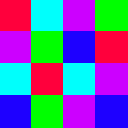
\includegraphics[width=0.9\linewidth]{./images/Nearest_Neighbour_Normal.png}
                    \caption{}
                    \label{fig:example_nearest_neighbour_normal}
                \end{subfigure}%DO NOT REMOVE THIS COMMENT
                \begin{subfigure}{.333\textwidth}
                    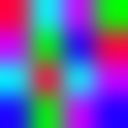
\includegraphics[width=0.9\linewidth]{./images/Nearest_Neighbour_Blur_10px.png}
                    \caption{}
                    \label{fig:example_nearest_neighbour_blur}
                \end{subfigure}%DO NOT REMOVE THIS COMMENT
                \begin{subfigure}{.333\textwidth}
                    \centering
                    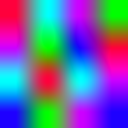
\includegraphics[width=0.9\linewidth]{./images/Nearest_Neighbour_Bicubic.png}
                    \caption{}
                    \label{fig:example_nearest_neighbour_bicubic}
                \end{subfigure}
                \caption{These figures show the similarities between applying a Gaussian Blur to a nearest neighbour interpolation, as seen in figure~\ref{fig:example_nearest_neighbour_blur}, and a bicubic filter, as seen in figure~\ref{fig:example_nearest_neighbour_bicubic}}
                \label{fig:example_nearest_neighbour}
            \end{figure}

            A possible improvement to nearest neighbour is to apply a convolution filter to the data such as that shown in figure~\ref{fig:example_nearest_neighbour}. In this figure we originally started with a 4 by 4 pixel image. Using a nearest neighbour algorithm we scaled this up to 128 by 128 pixels as seen in figure~\ref{fig:example_nearest_neighbour_normal}. When we apply a 10 pixel Gaussian Blur, a type of convolution filter, as in figure~\ref{fig:example_nearest_neighbour_blur}, we see that we achieve results similar to that of applying a bicubic interpolation algorithm as in figure~\ref{fig:example_nearest_neighbour_bicubic}. By varying the blur radius we may be able to achieve an algorithm tuned for particular types of data. 


        \subsubsection{Inverse Distance Weighting}\label{background_interpolation_methods_inverse_distance_weighting}

            The methodology of inverse distance weighting (IDW) is the calculation of new data points as the weighted average of neighbouring known data points. The weighting is calculated as the inverse of the distance from the current point to the neighbour currently being checked and are normalised such that the total weighting is equal to one. Due to the requirement of checking all other points the time complexity of this algorithm, like many other interpolation algorithms, is $O(n^{2})$. However it is possible to reduce this by some constant factor by imposing a maximum radius on all calculations, which also has the possibility of raising the accuracy of the algorithm. This radius is not used in this project and is therefore a candidate for future study.

            The general formula for calculating the value, $V$, at a point $X_{i}$, given known samples $S$, where $f(S_{i})$ is the value of sample $S$, is:

            \begin{align*}
                V = \sum_{i=1}^{N}{f(S_{i})\frac{w_{i}(X_{i})}{\sum_{j=0}^{N}{w_{j}(X_{j})}}}
            \end{align*}

            where 

            \begin{align*}
                w_{i}(x) = \frac{1}{d(x,S_{i})^{p}}
            \end{align*}

            is a weighting function with $d(X_{1},X_{2})$ being a distance metric between points $X_{1}$ and $X_{2}$, and $p$ is the power parameter, which controls the rate of change at which distances affect the weighting.

            \begin{figure}[H]
                \centering
                \begin{subfigure}{.5\textwidth}
                    \centering
                    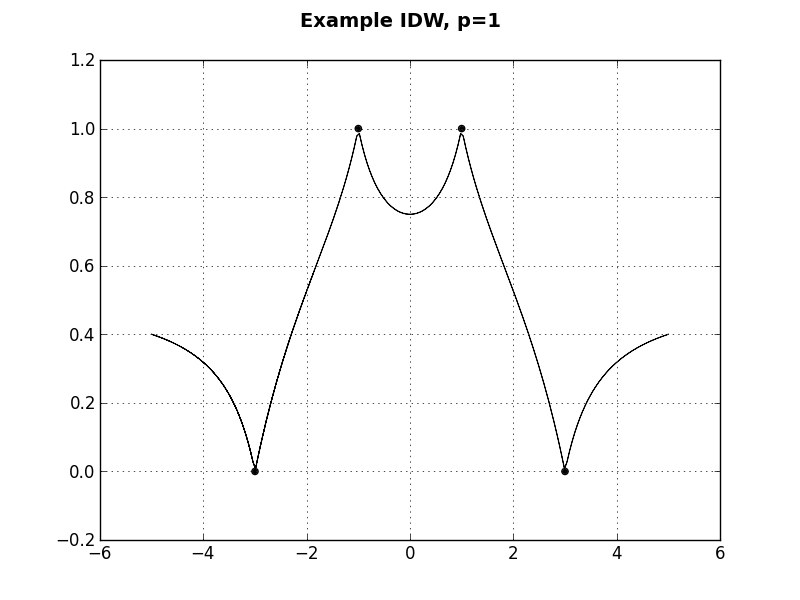
\includegraphics[width=\linewidth]{./images/IDWPF1.png}
                    \caption{}
                    \label{fig:example_idw_p1}
                \end{subfigure}%DO NOT REMOVE THIS COMMENT
                \begin{subfigure}{.5\textwidth}
                    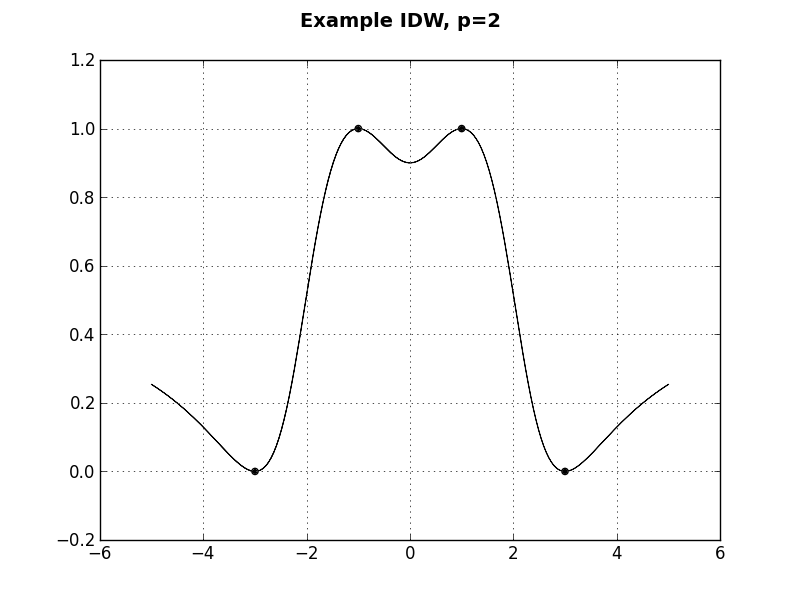
\includegraphics[width=\linewidth]{./images/IDWPF2.png}
                    \caption{}
                    \label{fig:example_idw_p2}
                \end{subfigure}
                \begin{subfigure}{.5\textwidth}
                    \centering
                    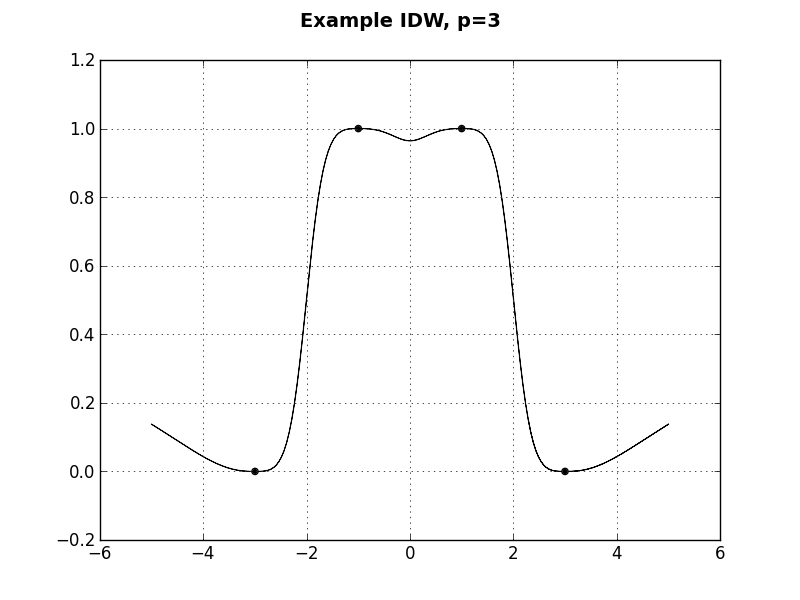
\includegraphics[width=\linewidth]{./images/IDWPF3.png}
                    \caption{}
                    \label{fig:example_idw_p3}
                \end{subfigure}%DO NOT REMOVE THIS COMMENT
                \begin{subfigure}{.5\textwidth}
                    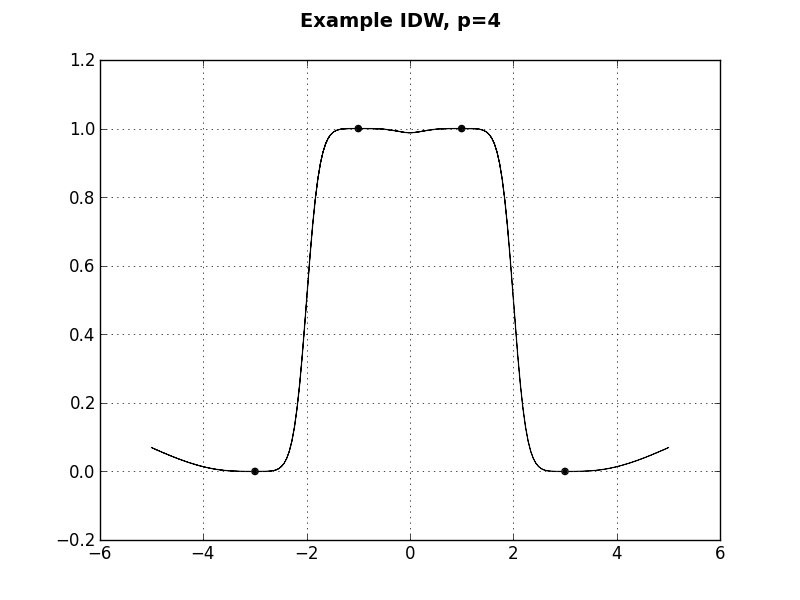
\includegraphics[width=\linewidth]{./images/IDWPF4.png}
                    \caption{}
                    \label{fig:example_idw_p4}
                \end{subfigure}
                \caption{These two figures show the IDW algorithm in one dimension at points -3,-1,1 and 3 where the values are 0,1,1 and 0 respectively. Figures~\ref{fig:example_idw_p1},~\ref{fig:example_idw_p2},~\ref{fig:example_idw_p3} and ~\ref{fig:example_idw_p4} have power parameters of 1,2,3 and 4 respectively.}
                \label{fig:example_idw}
            \end{figure}

            As we can see in figure~\ref{fig:example_idw_p1}, IDW's dependence on the surrounding values causes interesting effects. Between the x values of -1 and 1 we can see a local minima in the graph. This is due to the fact that the values at -3 and 3 are lower and are taken into account. A way of mitigating this effect is to increase the power parameter as has been done in figures~\ref{fig:example_idw_p2},~\ref{fig:example_idw_p3} and ~\ref{fig:example_idw_p4}. It should be noted that as the power parameter goes to infinity, the IDW algorithm approaches the nearest neighbour algorithm. 

            A further example of this effect is figure~\ref{fig:example_idw_distance}, which has the extreme values further away, causing the local minima, at the location $x = 0$, to be less pronounced.

            \centerimage{.5\textwidth}{./images/IDW_distance.png}{A modification of figure~\ref{fig:example_idw_p2} which demonstrates how moving the extreme points further from zero by a value of one, affects the interpolation.}{fig:example_idw_distance}


        \subsubsection{Natural Neighbour}\label{background_interpolation_methods_natural_neighbour}

            Natural neighbour interpolation is based on Voronoi tessellation~\cite{multivariatedata}. The basic method is very similar to that of IDW in that the basic form of the equation is:

            \begin{align*}
                G(x,y) = \sum_{i=1}^{n}{w_{i}f(x_{i},y_{i})}, 
            \end{align*}

            where $w_{i}$ is the weighting factor and $f(x_{i},y_{i})$ is the value at known point $(x_{i},y_{i})$. The main difference between natural neighbour and IDW is the method used to calculate the weighing. In natural neighbour the weighting is calculated as the ratio of area of the new region that originally belonged to the current known point in a Voronoi diagram. As such all weightings sum to one, which ensures that the original values do not change. An example of this can be seen in figure~\ref{fig:natural_neighbour}. 

            \centerimageanywhere{0.4\textwidth}{./images/Natural_Neighbour.png}{An illustration of the method for calculating the weighing in natural neighbour. This figure was created by Wikipedia user \emph{Markluffel}.}{fig:natural_neighbour}

    \subsection{Regular Grid Algorithms}\label{background_interpolation_methods_regulargrid}

        Regular grid algorithms require the known data points to be on a regular grid. This can be achieved with irregular data by making the grid sufficiently large and ``snapping'' data points to it.

        \subsubsection{Bilinear}\label{background_interpolation_methods_bilinear}

            Bilinear interpolation, is the simplest of the grid interpolation algorithms which will be evaluated. The algorithm is the two dimensional equivalent of linear interpolation, and works by evaluating the linear interpolation in both the x and y directions and combining them. Essentially this calculates each points as a weighted average of the nearest point in each direction. This algorithm is originally used in images, where the nearest points are pixels. 

            The main disadvantage of bilinear interpolation is that if there is an outlier point nearby then this has a large effect on interpolated points and there is no way of controlling this. It also has the disadvantage that it cannot extrapolate any information. All points to be interpolated must be inside the convex hull of the known points.


        \subsubsection{Bicubic}\label{background_interpolation_methods_bicubic}

            Bicubic interpolation, a popular algorithm in image resampling, is essentially an improved version of bilinear interpolation, when applied to images. As a cubic Hermite spline~\cite{practicalguidesplines}, the output is smoother than linear interpolation, as we can see in figure~\ref{fig:bicubic_vs_bilinear}. The bicubic algorithm achieves this by taking into account the 16 points surrounding the point to be interpolated rather than just 4. 

            \begin{figure}[H]
                \centering
                \begin{subfigure}{.5\textwidth}
                    \centering
                    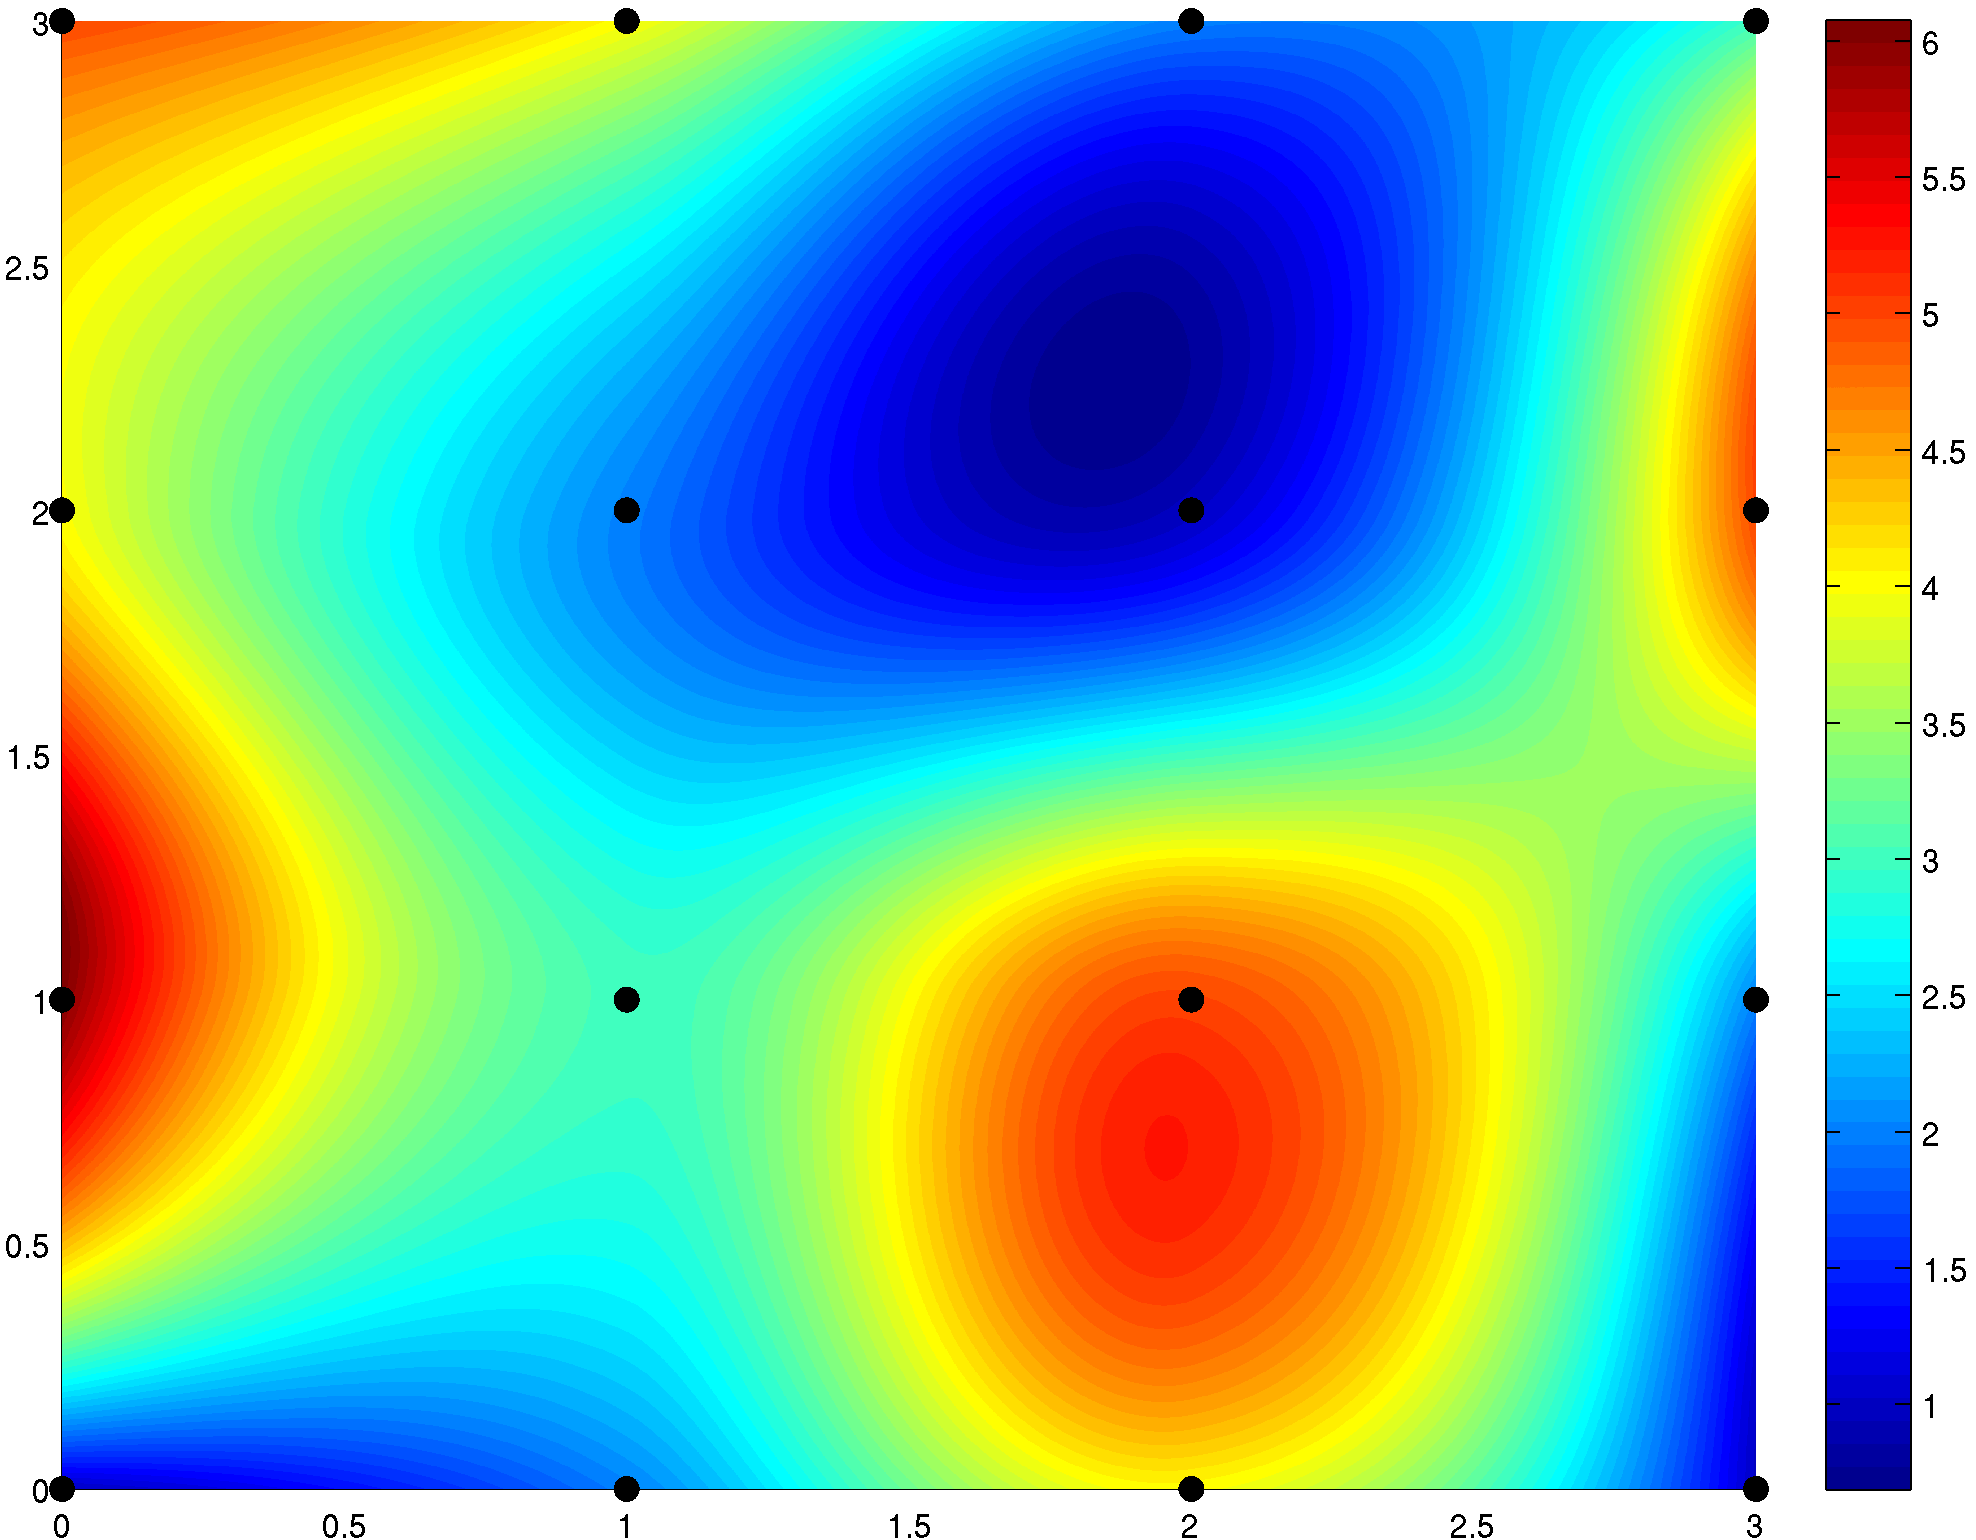
\includegraphics[width=0.9\linewidth]{./images/Bicubic_Interpolation_Example.png}
                    \caption{}
                    \label{fig:example_bicubic}
                \end{subfigure}%DO NOT REMOVE THIS COMMENT
                \begin{subfigure}{.5\textwidth}
                    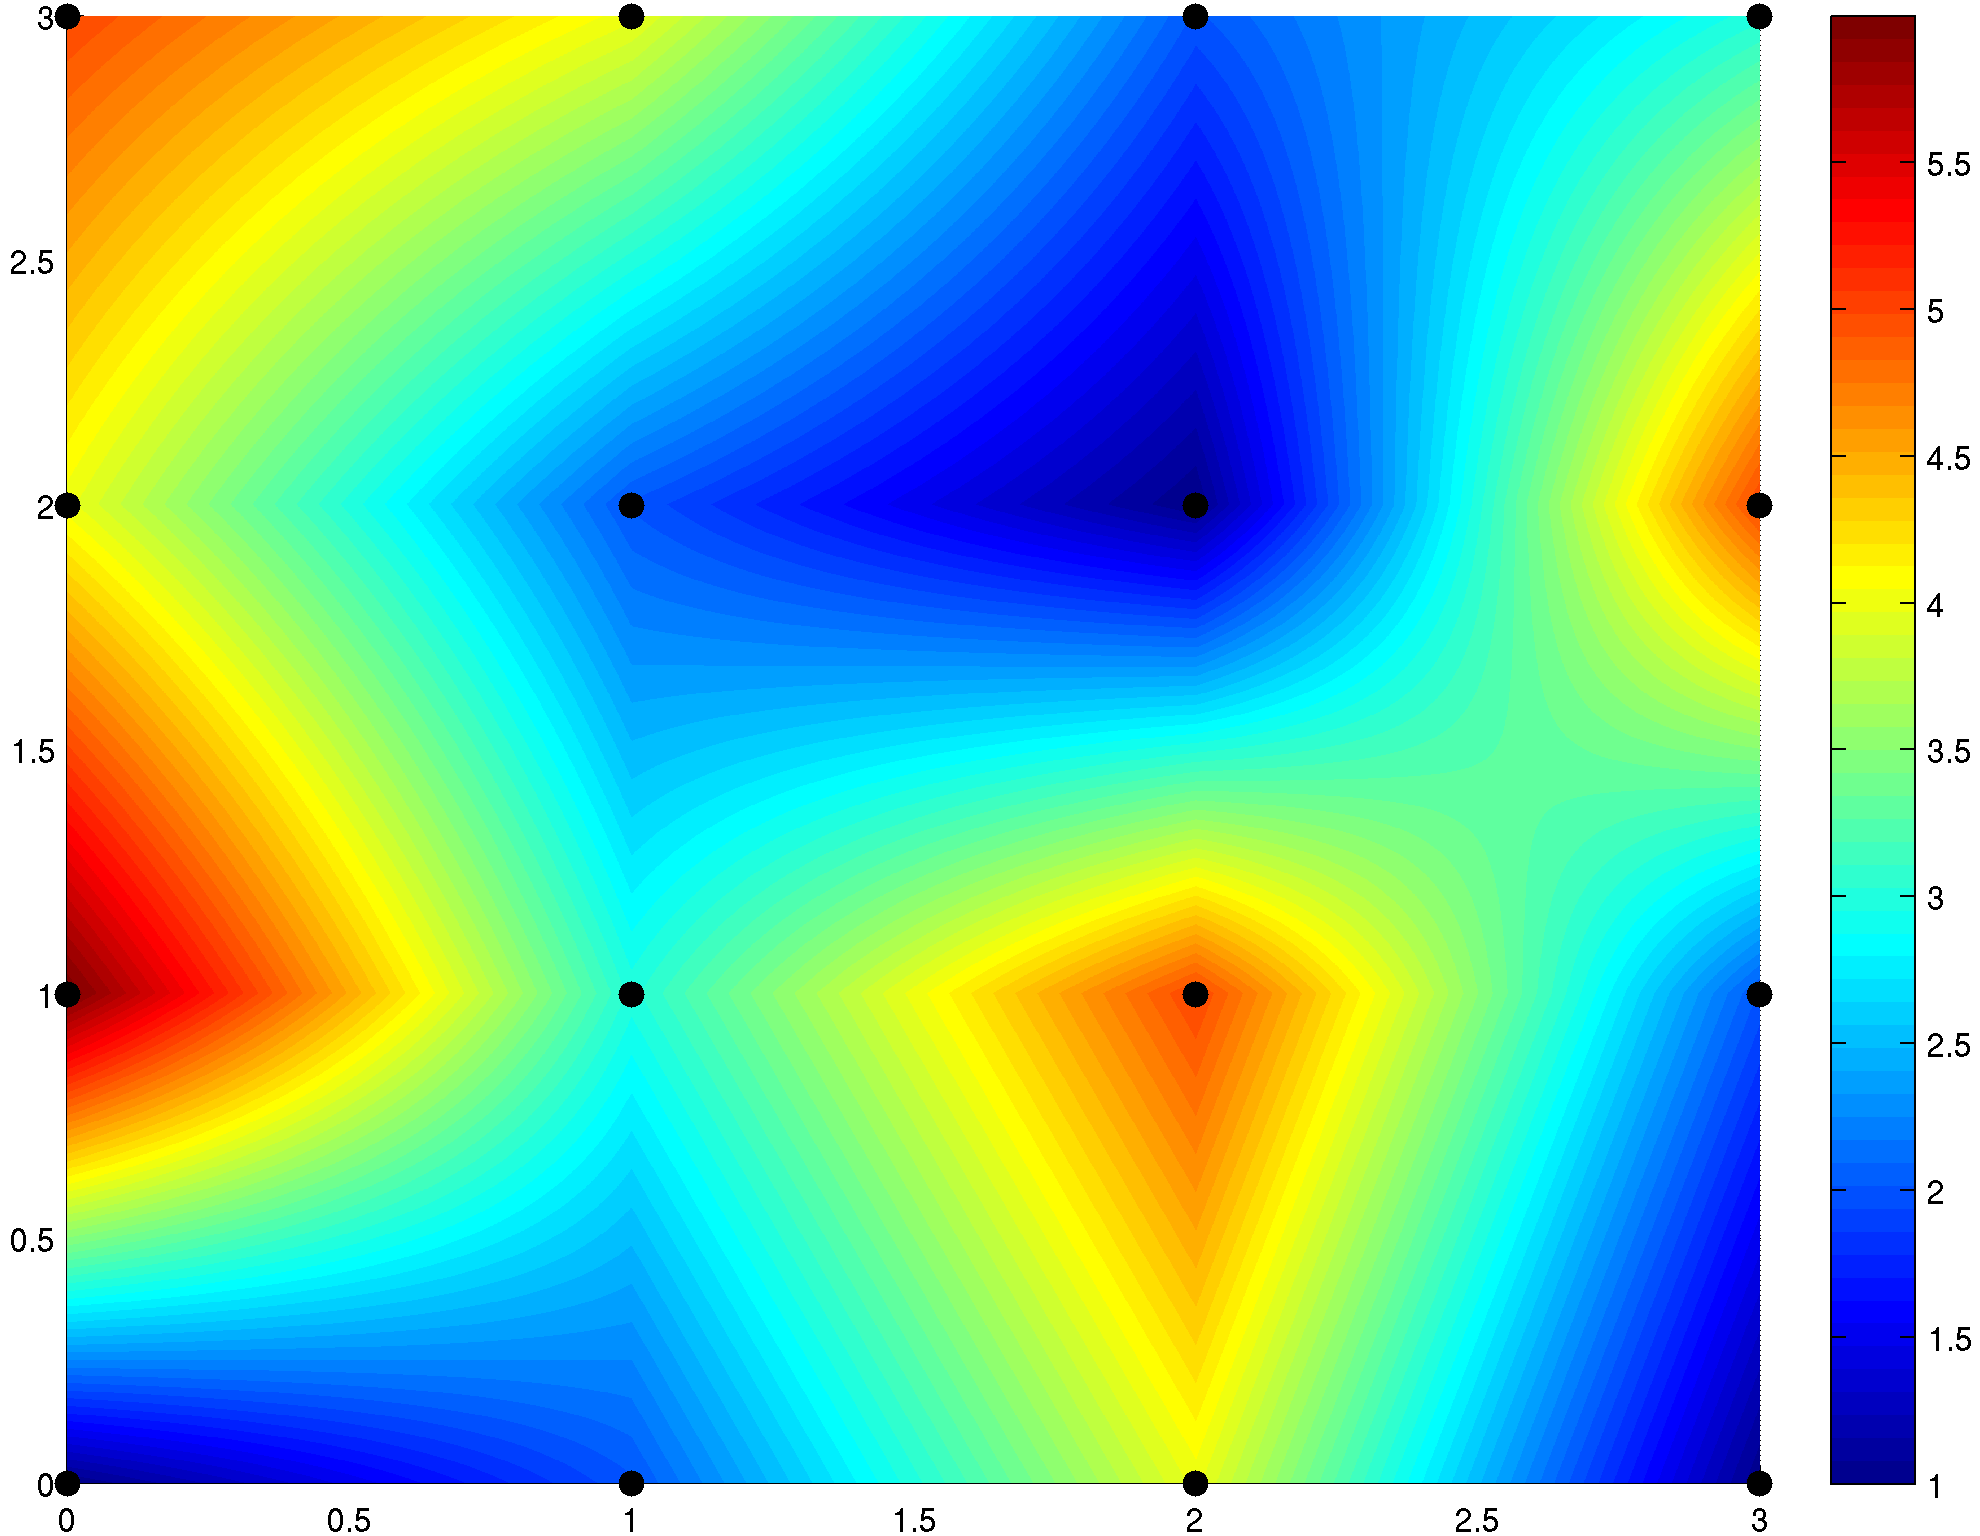
\includegraphics[width=0.9\linewidth]{./images/Bilinear_Interpolation_Example.png}
                    \caption{}
                    \label{fig:example_bilinear}
                \end{subfigure}
                \caption{The difference between bicubic interpolation, figure~\ref{fig:example_bicubic}, and bilinear interpolation, figure~\ref{fig:example_bilinear}, on the same dataset. These examples were created by Wikipedia user \emph{Berland}.}
                \label{fig:bicubic_vs_bilinear}
            \end{figure}

            The algorithm for bicubic interpolation is more complicated than that of bilinear interpolation, requiring the solution to a system of linear equations~\cite{bicubicorigins}, but also cannot extrapolate, only interpolate. 

        \subsubsection{Barnes}\label{background_interpolation_methods_barnes}

            Barnes interpolation uses a multi-pass approach to determine the new data points. The method has found success in calculating air pressure across the United States, providing results similar to measured data, however it depends on the data points be reasonably uniform~\cite{barnesinterpolation}.

            The algorithm works by calculating a simple distance weighted interpolation as the first result, and then iterating multiple times using a calculated error field to reduce the errors in the output. 

            One important factor in Barnes interpolation is the fact that it depends on several constants. These constants depend on the type of data being interpolated and the nature of the measurements, including the density of the measurements. As such, determining these constants is a key part of using this algorithm for interpolation. One advantage of this approach, is that we can iterate over our data set and tune it to the known measurements in order to make sure it is as accurate as possible. Experiments using this algorithm have used similar mechanisms and shown success~\cite{pmconcentrationmaps}.

            The algorithm for Barnes interpolation is as follows.

            For the first pass each known point is assigned a weight using the formula: 

            \begin{align*}
                W_{i} &= e^{-(d/R^{2})}
            \end{align*}
            
            where d is the distance between the known point and the current point to be interpolated, and R is the radius of influence. Using this weight, the initial estimates of the unknown points are calculated as: 
            
            \begin{align*}
                X_{g} &= \frac{\sum_{i}{W_{i}X_{i}}}{\sum_{i}{W_{i}}}
            \end{align*}

            At this point we begin our successive passes. These are defined as:

            \begin{align*}
                X'_{g} &= X_{g} + \frac{\sum_{i}{W'_{i}E_{i}}}{\sum_{i}{W'_{i}}}
            \end{align*}

            where $E_{k}$ is the difference between the estimated value and the actual value at a known point $k$ and $W'_{i}$ is defined as:

            \begin{align*}
                W'_{i} &= e^{-(d/\Gamma R)^{2}}
            \end{align*}

            with $\Gamma$ as a convergence parameter normally set in the range 0.2-0.3. In our experiments we will use the recommended value of 0.29 in order to limit the effects of dimensionality.


